\subsection*{Model}

\begin{frame}[fragile]{Problem presentation}

\begin{columns}
\begin{column}{0.5\textwidth}
\only<2>{\includegraphics[scale=0.3]{mixCode1-5.pdf}}
\only<3->{\paragraph{Basic idea :}\\
 "Expert" threshold $s$ \\  
 $$ State_i=1 \quad \mbox{if} Y_i<s$$
 $$ State_i=2 \quad \mbox{if} Y_i\geq  s $$
}
\only<5->{\paragraph{Improvement:}\\
 \textcolor{blue}{Estimating} the threshold s and  reconstruction of the hidden state (colour)\\
 Compute the \textcolor{blue}{probability to belong} to State 1 or 2.\\
}
 \only<6->{
 \bigskip
   \centering{$\Longrightarrow$ \textcolor{red}{Mixture Model}}
 }
 \end{column}
 \begin{column}{0.4\textwidth}

 \only<1>{\includegraphics[scale=0.3]{mixCode1-1.pdf}}
 \only<2>{\includegraphics[scale=0.3]{mixCode1-2.pdf}}
 \only<3>{\includegraphics[scale=0.3]{mixCode1-3.pdf}}
 \only<4->{\includegraphics[scale=0.3]{mixCode1-4.pdf}}
\end{column}
\end{columns}
\end{frame}

%%-----------------------------------------------------------------%%
%%-----------------------------------------------------------------%%

\begin{frame}[fragile]{Proposed model}
\paragraph{Model}
For a given number of states $K$, 

\begin{itemize}
\item
%  \blue{Modelling $Z$}: $\pi_k=\P(Z_i=k), \quad k=1,\ldots, K, \quad \sum_k \pi_k=1$\par
%  $Z_i \overset{i.i.d}{\sim} \Mcal(1, \pibf), \quad P(Z_{ik}=1)=\pi_k$
%  \item \blue{Modelling $Y$}: The $Y_i's$ are assumed to be independent  conditionnaly to $\Zbf$ : $(Y_i\vert Z_i = k) \overset{i.i.d}{\sim} f_{\gamma_k}().$
\end{itemize}

 \onslide<2->{\centering{\blue{Model parameters $\thetabf =(\pibf, \gammabf)$}}\par}
 \onslide<3->{\centering{\includegraphics[scale=0.4]{Dag2.pdf}}}
\end{frame}

\begin{frame}[fragile]{Proposed model}
\paragraph{Model}
For a given number of states $K$, 
\begin{itemize}
\item
 \blue{Modelling $Z$}: $\pi_k=\P(Z_i=k), \quad k=1,\ldots, K, \quad \sum_k \pi_k=1$\par
 $Z_i \overset{i.i.d}{\sim} \Mcal(1, \pibf)$
 \item \blue{Modelling $Y$}: The $Y_i's$ are assumed to be independent  conditionnaly to $\Zbf$ : $(Y_i\vert Z_i = k) \overset{i.i.d}{\sim} f_{\gamma_k}().$
\end{itemize}
\begin{columns}
  \begin{column}{0.45\textwidth}
\begin{knitrout}
\definecolor{shadecolor}{rgb}{0.969, 0.969, 0.969}\color{fgcolor}\begin{kframe}
\begin{alltt}
\hlstd{K} \hlkwb{<-} \hlnum{2}\hlstd{; N} \hlkwb{<-} \hlnum{100}\hlstd{; mu} \hlkwb{<-} \hlkwd{c}\hlstd{(}\hlnum{3}\hlstd{,} \hlnum{7}\hlstd{); sigma} \hlkwb{<-} \hlkwd{c}\hlstd{(}\hlnum{1}\hlstd{,}\hlnum{1.5}\hlstd{)}
\hlstd{Z} \hlkwb{<-} \hlkwd{sample}\hlstd{(}\hlnum{1}\hlopt{:}\hlnum{2}\hlstd{,} \hlkwc{size} \hlstd{= N,} \hlkwc{replace}\hlstd{=T,} \hlkwc{prob}\hlstd{=}\hlkwd{c}\hlstd{(}\hlnum{0.3}\hlstd{,} \hlnum{0.7}\hlstd{))}
\hlkwd{plot}\hlstd{(Z,} \hlkwc{col}\hlstd{=Z}\hlopt{+}\hlnum{1}\hlstd{,} \hlkwc{pch}\hlstd{=}\hlnum{15}\hlstd{,} \hlkwc{cex}\hlstd{=}\hlnum{0.3}\hlstd{)}
\hlstd{Y.mixture} \hlkwb{<-} \hlkwd{rnorm}\hlstd{(N,} \hlkwc{mean}\hlstd{=mu[Z],} \hlkwc{sd}\hlstd{=sigma[Z])}
\hlkwd{plot}\hlstd{(Y.mixture,} \hlkwc{col}\hlstd{=Z}\hlopt{+}\hlnum{1}\hlstd{,} \hlkwc{pch}\hlstd{=}\hlnum{19}\hlstd{)}
\end{alltt}
\end{kframe}
\end{knitrout}
 \end{column}
  \begin{column}{0.45\textwidth}
    \only<3>{\includegraphics[height=3cm, width=6cm]{mixCode2-1.pdf}}
    \only<4->{\includegraphics[scale=0.25]{mixCode2-2.pdf}}
  \end{column}
  \end{columns}
\end{frame}

\begin{frame}[fragile]{Model Properties}
\begin{itemize}
\item Couples $\{(Y_i, Z_i)\}$ are i.i.d.
\item \blue{Label switching}:\\ the model is invariant for any permutation of the labels $\{1,
  \dots, K\}$ $\Rightarrow$ the mixture model has \emphase{$K!$
    equivalent definitions}.
\item\blue{Distribution of a $Y_i$:}\\
$$P(Y_i)=\sum_{k=1}^K P(Y_i, Z_i=k)=\textcolor{blue}{P(Z_i=k)} \textcolor{magenta}{P(Y_i | Z_i=k)} $$
\item\blue{Distribution of $\Ybf$:}\\
{\small
\begin{eqnarray*}
P(\Ybf ; \thetabf, \pibf)= \prod_{i=1}^n \sum_{k=1}^K P(Y_i , Z_i=k)  
&=& \prod_{i=1}^n \sum_{k=1}^K \textcolor{blue}{P(Z_i=k)} \textcolor{magenta}{P(Y_i | Z_i=k)} \\ 
&=& \prod_{i=1}^n \sum_{k=1}^K \textcolor{blue}{\pi_k} \textcolor{magenta}{f_{\gamma_k}(Y_i)} 
\end{eqnarray*}
}
\end{itemize}
\end{frame}

\subsection*{Parameter estimation}
%%-----------------------------------------------------------------%%
%%-----------------------------------------------------------------%%


\begin{frame}{Statistical inference of incomplete data models} 
 \paragraph{Maximum likelihood estimate:} We are looking for
  $$
  (\widehat{\thetabf},\widehat{\pibf}) = \arg\max_{\thetabf, \pibf} \log P(\Ybf; \thetabf, \pibf)
  $$
  \begin{itemize}
  \item Likelihood of the observed data (or observed likelihood):
    $$
    \log P(\Ybf; \thetabf, \pibf)=
    \sum_{i=1}^n \log \left[\sum_{k=1}^K \pi_k f_{ \gamma_k}(Y_i)\right]
    $$
  \item No analytical estimators. 
%  \item  It is not always possible since this sum typically involves $K^n$ terms : $2^{100}\approx10^{30}$, the computation will take $10^{10}$ years on a 2014 computer. 
  \item Brute force algorithm is not the way
  \end{itemize}
\end{frame}
%%-----------------------------------------------------------------%%
%%-----------------------------------------------------------------%%


\begin{frame}{And what if $\Zbf$ were observed  ?}
The complete likelihood is 
\begin{align*}
    \log P(\Ybf, \Zbf; \thetabf, \pibf) &=\log P(\Zbf; \pibf) + \log P(\Ybf\vert \Zbf; \thetabf)\\
      & =  \sum_i \sum_k Z_{ik} \log \pi_k + \sum_i \sum_k Z_{ik} \log
    f_{\gamma_k}(Y_i) \\
    & =  \sum_i \sum_k Z_{ik} [\log \pi_k + \log
      f_{\gamma_k}(Y_i)].
\end{align*}
  
Now, the sum contains $nK$ ($200$ if $n=100$ and $K=2$) terms.  It is much easier.
\pause

\centering{\textcolor{red}{Unfortunately $\Zbf$ are unknown.} }
\pause

\bigskip

\textcolor{red}{Idea:} Replace $Z_i$, by our best guess, that is~:
% $$
% \tau_{ik}:=\Esp(Z_i = k | Y_i)=P(Z_i = k | Y_i)
% $$  
\end{frame}

\begin{frame}{Idea of EM algorithm}
% $$     =  \sum_i \only<1>{\sum_k Z_{ik}}\only<2>{\textcolor{red}{\tau_{ik}} } [\log \pi_k + \log
%       f_{\gamma_k}(Y_i)].
% $$
% \only<2>{where $\tau_{ik}$ is a good approximation of $Z_{ik}$.}
% 
% \only<3> If parameter $\thetabf_0$ is known, a good approximation is $\tau_{ik}^{(0)}=\Esp_{\thetabf}\left\lbrace Z_{ik}\vert \Ybf\right\rbrace$.
% 
% \only<4> Idea : iterative algorithm, for a value of $\thetabf^{(l)}$, compute $\tau_{ik}^{(l)}$, and then update $\thetabf^{(l)}$ to $\thetabf^{(l)}$. 
\end{frame}


\begin{frame}{More generally - EM algorithm}
\begin{columns}
\begin{column}{0.2\textwidth}
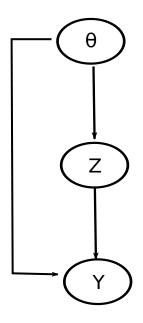
\includegraphics[scale=0.5]{ModHier.pdf}
\end{column}
\begin{column}{0.8\textwidth}
\paragraph{Bayes Formula}
{\small
\begin{align*}
P(\Ybf, \Zbf;\thetabf) & = P(\Ybf\vert \Zbf; \thetabf) P(\Zbf; \thetabf),\\
& = \textcolor{orange}{P(\Zbf\vert \Ybf; \thetabf) P(\Ybf; \thetabf).}
\end{align*}
Therefore,
\begin{align*}
\log P(\Ybf; \thetabf) & = \log \left \lbrace P(\Ybf, \Zbf;\thetabf) / P(\Zbf\vert \Ybf; \thetabf) \right\rbrace\\
& = \log P(\Ybf, \Zbf;\thetabf) - \log P(\Zbf\vert \Ybf; \thetabf) \\
\end{align*}
For a given $\thetabf_0$, we may compute $P_{\thetabf_0}=P(\Zbf\vert \thetabf_0, \Ybf)$ and
\begin{align*}
\log P(\Ybf; \thetabf) &= \Esp_{\thetabf_0}(\log P(\Ybf, \Zbf;\thetabf)) - \Esp_{\thetabf_0}(\log P(\Zbf\vert \Ybf; \thetabf))\\
  & = Q(\thetabf, \thetabf_0) - H(\thetabf, \thetabf_0)
  \end{align*}}
\end{column}
\end{columns}
\end{frame}


\begin{frame}{More generally - EM algorithm}
\begin{columns}
\begin{column}{0.2\textwidth}
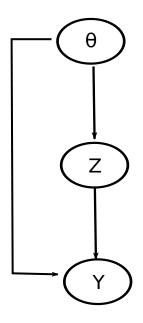
\includegraphics[scale=0.5]{ModHier.pdf}
\end{column}
\begin{column}{0.8\textwidth}
{\small
Since 
$$\log P(\Ybf; \thetabf)  = Q(\thetabf, \thetabf_0) - H(\thetabf, \thetabf_0),$$
and $H(\thetabf, \thetabf_0)$ achieves its maximum in $\thetabf_0$,
\begin{align*}
\log P(\Ybf; \thetabf)- \log P(\Ybf; \thetabf_0)  = & \textcolor{orange}{(Q(\thetabf, \thetabf_0) - Q(\thetabf, \thetabf_0))} +\cr
&\textcolor{green}{(H(\thetabf_0, \thetabf_0)-H(\thetabf, \thetabf_0))}.
\end{align*}
}

\paragraph{Expectation - Maximization algorithm}
\begin{enumerate}
\item Phase E : \\
Calculate  $Q(\thetabf,\thetabf^{k})$ for every $\thetabf$.
\item Phase M :\\ Define  
$\thetabf^{k+1}=argmax\, Q(\thetabf,\thetabf^{k})$
\end{enumerate}
\end{column}
\end{columns}
\end{frame}

\begin{frame}{EM algorithm for independent mixture model}
\begin{align*}
  Q(\thetabf,\thetabf^{(\ell)}) & = \Esp_{\thetabf^{(\ell)}}(\log P(\Ybf, \Zbf;\thetabf))\\
  &= \Esp_{\thetabf^{(\ell)}} \left\{\sum_i \sum_k Z_{ik} [\log \pi_k + \log
       f_{\gamma_k^{(\ell)}}(Y_i)] \right\}\\
  &= \sum_i \sum_k \Esp_{\thetabf^{(\ell)}} (Z_i = k | Y_i) \log\left[\pi_k f_{\gamma_k^{(\ell)}}(Y_i)\right]
  \end{align*}
   Recall that $\tau_{ik}^{(\ell)}:=P_{\thetabf^{(\ell)}}(Z_i = k | Y_i )$
   $$Q(\thetabf;\thetabf^{(\ell)})
     =\sum_i \sum_k \tau_{ik}^{(\ell)} \log \pi_k +  \sum_i \sum_k \tau_{ik}^{(\ell)}\log f_{\gamma_k^{(\ell)}}(Y_i)$$
     $\rightarrow$ Need to estimate $\tau_{ik}^{(\ell)}$
\end{frame}

\begin{frame}{EM algorithm for independent mixture model}
    \begin{itemize}
    \item Initialisation of $\thetabf^{(0)}=(\pi_1, ..., \pi_K, \gamma_1, ..., \gamma_K)^{(0)}$.
  \pause
  \item Alternate  
      \begin{description}
      \item[E-step] Calculation of $\tau^{(\ell)}_{ik}=P(Z_i = k | y_i, \thetabf^{(\ell-1)}) = \frac{\pi^{(\ell-1)}_k f_{\theta^{(\ell-1)}_k}(y_i)}{\sum_{k'} \pi^{(\ell-1)}_{k'}f_{\theta^{(\ell-1)}_{k'}}(x_i)}$

      \item[M-step] Maximization of
        $$
        (\pibf, \gammabf) \longmapsto \sum_i \sum_k \tau_{ik}^{(\ell)} [\log \pi_k +
          \log f(x_i; \gamma_k)]
        $$
      \end{description} 
    \end{itemize}
\end{frame}

\begin{frame}{In our situation}
\begin{itemize}  
\item $Z \in \{1,2\}$: $P(Z=1)=\pi_1$ and $P(Z=2)=1-\pi_1$  
\item For $k=1$ or $2$, $(X|Z=k) \sim \Ncal(\mu_k, \sigma_k^2)$ 
\item the parameter vector is $(\pi, \mu_1, \mu_2, \sigma_2^2, \sigma_2^2)$
\item[] Assume that $n$ observations $y_1, y_2, ..., y_n$ are available
\item The parameter estimators  at step $(\ell+1)$ of the EM algorithm 
are given by:
\end{itemize}
\bigskip
   \begin{eqnarray*}
     \widehat{\pi}_1^{(\ell+1)} & = & \frac1{n} \sum_{i=1}^n \tau_{i1} ^{(\ell)}, \\
     \widehat{\mu}_k^{(\ell+1)} & = & \frac1{\sum_{i=1}^n  \tau_{ik} ^{(\ell)}} \sum_{i=1}^n \tau_{ik}^{(\ell)} y_i \\ 
     \widehat{\sigma}^2_{k^{(\ell+1)}} & = &  \frac1{\sum_{i=1}^n  \tau_{ik} ^{(\ell)}} \sum_{i=1}^n \tau_{ik}^{(\ell)} (y_i - \widehat{\mu}_k^{(\ell)})^2
  \end{eqnarray*}
   $\rightarrow$ They are a \emphase{weighted version} of the usual maximum
   likelihood estimates. 
\end{frame}


\begin{frame}[fragile]{Back on earth - Practically speaking}
\begin{columns}
\begin{column}{0.5\textwidth}
\begin{knitrout}
\definecolor{shadecolor}{rgb}{0.969, 0.969, 0.969}\color{fgcolor}\begin{kframe}
\begin{alltt}
\hlcom{#library('mclust')}
\hlkwd{library}\hlstd{(}\hlstr{'mixtools'}\hlstd{)}
\end{alltt}


{\ttfamily\noindent\itshape\color{messagecolor}{\#\# Loading required package: boot\\\#\# Loading required package: MASS\\\#\# Loading required package: segmented\\\#\# mixtools package, version 1.0.2, Released May 14 2014\\\#\# This package is based upon work supported by the National Science Foundation under Grant No. SES-0518772.}}\begin{alltt}
\hlstd{Y.clustering} \hlkwb{<-} \hlkwd{normalmixEM} \hlstd{(Y.mixture,} \hlkwc{lambda} \hlstd{=} \hlkwa{NULL}\hlstd{,} \hlkwc{mu} \hlstd{=} \hlkwa{NULL}\hlstd{,} \hlkwc{sigma} \hlstd{=} \hlkwa{NULL}\hlstd{,} \hlkwc{k} \hlstd{=} \hlnum{2}\hlstd{,}
                             \hlkwc{mean.constr} \hlstd{=} \hlkwa{NULL}\hlstd{,} \hlkwc{sd.constr} \hlstd{=} \hlkwa{NULL}\hlstd{,}
                             \hlkwc{epsilon} \hlstd{=} \hlnum{1e-07}\hlstd{,} \hlkwc{maxit} \hlstd{=} \hlnum{1000}\hlstd{,} \hlkwc{maxrestarts}\hlstd{=}\hlnum{20}\hlstd{)}
\end{alltt}
\begin{verbatim}
## number of iterations= 94
\end{verbatim}
\begin{alltt}
\hlkwd{summary}\hlstd{(Y.clustering)}
\end{alltt}
\begin{verbatim}
## summary of normalmixEM object:
##          comp 1   comp 2
## lambda 0.644837 0.355163
## mu     7.366618 3.072069
## sigma  1.374730 1.142811
## loglik at estimate:  -220.6712
\end{verbatim}
\begin{alltt}
\hlstd{Y.clustering}\hlopt{$}\hlstd{posterior}
\end{alltt}
\begin{verbatim}
##              comp.1       comp.2
##   [1,] 0.9969687292 3.031271e-03
##   [2,] 0.9851514346 1.484857e-02
##   [3,] 0.9997121657 2.878343e-04
##   [4,] 0.0161326028 9.838674e-01
##   [5,] 0.9999512614 4.873864e-05
##   [6,] 0.9999999696 3.042552e-08
##   [7,] 0.0005076365 9.994924e-01
##   [8,] 0.9579043973 4.209560e-02
##   [9,] 0.9998855989 1.144011e-04
##  [10,] 0.9951533652 4.846635e-03
##  [11,] 0.2786839900 7.213160e-01
##  [12,] 0.0059443996 9.940556e-01
##  [13,] 0.9999836329 1.636709e-05
##  [14,] 0.0368165290 9.631835e-01
##  [15,] 0.9971375143 2.862486e-03
##  [16,] 0.0028544586 9.971455e-01
##  [17,] 0.9755156762 2.448432e-02
##  [18,] 0.0005989360 9.994011e-01
##  [19,] 0.9999835040 1.649601e-05
##  [20,] 0.9975125295 2.487470e-03
##  [21,] 0.9999999764 2.360440e-08
##  [22,] 0.9547557394 4.524426e-02
##  [23,] 0.8695335538 1.304664e-01
##  [24,] 0.9994090331 5.909669e-04
##  [25,] 0.1078727174 8.921273e-01
##  [26,] 0.0019725859 9.980274e-01
##  [27,] 0.9999756303 2.436966e-05
##  [28,] 0.9825448057 1.745519e-02
##  [29,] 0.9999955154 4.484646e-06
##  [30,] 0.9949524424 5.047558e-03
##  [31,] 0.9977340618 2.265938e-03
##  [32,] 0.3844070691 6.155929e-01
##  [33,] 0.6358648909 3.641351e-01
##  [34,] 0.9986272956 1.372704e-03
##  [35,] 0.0014388339 9.985612e-01
##  [36,] 0.9979728669 2.027133e-03
##  [37,] 0.9999999235 7.654293e-08
##  [38,] 0.0001195139 9.998805e-01
##  [39,] 0.9995721112 4.278888e-04
##  [40,] 0.9992528007 7.471993e-04
##  [41,] 0.3606308191 6.393692e-01
##  [42,] 0.1978326093 8.021674e-01
##  [43,] 0.0021924454 9.978076e-01
##  [44,] 0.9952801499 4.719850e-03
##  [45,] 0.4327334801 5.672665e-01
##  [46,] 0.1348679072 8.651321e-01
##  [47,] 0.9999986008 1.399150e-06
##  [48,] 0.9999995851 4.149282e-07
##  [49,] 0.9999915740 8.426048e-06
##  [50,] 0.9990837930 9.162070e-04
##  [51,] 0.9863232129 1.367679e-02
##  [52,] 0.9644804877 3.551951e-02
##  [53,] 0.0178305291 9.821695e-01
##  [54,] 0.0017412448 9.982588e-01
##  [55,] 0.0023401499 9.976599e-01
##  [56,] 0.0040029722 9.959970e-01
##  [57,] 0.9998614798 1.385202e-04
##  [58,] 0.9999949343 5.065728e-06
##  [59,] 0.0002400381 9.997600e-01
##  [60,] 0.9999888883 1.111170e-05
##  [61,] 0.0021417526 9.978582e-01
##  [62,] 0.0058570692 9.941429e-01
##  [63,] 0.5585159804 4.414840e-01
##  [64,] 0.9998211910 1.788090e-04
##  [65,] 0.9245787218 7.542128e-02
##  [66,] 0.9968166992 3.183301e-03
##  [67,] 0.9901165941 9.883406e-03
##  [68,] 0.9990678607 9.321393e-04
##  [69,] 0.0004634915 9.995365e-01
##  [70,] 0.9999950954 4.904605e-06
##  [71,] 0.0044672843 9.955327e-01
##  [72,] 0.9999985457 1.454318e-06
##  [73,] 0.3302920680 6.697079e-01
##  [74,] 0.8554304063 1.445696e-01
##  [75,] 0.0015771278 9.984229e-01
##  [76,] 0.0457297999 9.542702e-01
##  [77,] 0.9999955288 4.471173e-06
##  [78,] 0.9995411383 4.588617e-04
##  [79,] 0.0092178203 9.907822e-01
##  [80,] 0.9973761089 2.623891e-03
##  [81,] 0.0231626465 9.768374e-01
##  [82,] 0.9998876875 1.123125e-04
##  [83,] 0.9963539491 3.646051e-03
##  [84,] 0.4130461972 5.869538e-01
##  [85,] 0.9999990052 9.947674e-07
##  [86,] 0.0048366542 9.951633e-01
##  [87,] 0.7363720205 2.636280e-01
##  [88,] 0.9999988876 1.112355e-06
##  [89,] 0.0245643657 9.754356e-01
##  [90,] 0.0229954032 9.770046e-01
##  [91,] 0.2286765833 7.713234e-01
##  [92,] 0.9999230264 7.697356e-05
##  [93,] 0.9999533083 4.669174e-05
##  [94,] 0.0814809684 9.185190e-01
##  [95,] 0.9999999203 7.972281e-08
##  [96,] 0.9998685558 1.314442e-04
##  [97,] 0.9991783228 8.216772e-04
##  [98,] 0.9987997820 1.200218e-03
##  [99,] 0.9998938166 1.061834e-04
## [100,] 0.9616710098 3.832899e-02
\end{verbatim}
\begin{alltt}
\hlstd{map} \hlkwb{<-}  \hlkwd{apply}\hlstd{(Y.clustering}\hlopt{$}\hlstd{posterior,}\hlnum{1}\hlstd{,which.max)}
\end{alltt}
\end{kframe}
\end{knitrout}
\end{column}
\begin{column}{0.5\textwidth}
\end{column}
\end{columns}
\end{frame}

\subsubsection*{Assumptions}
\subsection*{Example}
\subsection*{Theoretical aspects}
